\documentclass[10pt,letterpaper]{article}
\usepackage[utf8]{inputenc}
\usepackage[spanish,mexico]{babel}
\usepackage{amsmath}
\usepackage{amsfonts}
\usepackage{amssymb}
\usepackage{graphicx}
\usepackage{marvosym}
\usepackage{wrapfig}
\usepackage{breqn}
\usepackage{lalo}
\usepackage{hyperref}
\usepackage[left=2cm,right=2cm,top=2cm,bottom=2cm]{geometry}
\title{Informe de actividades}
\date{lunes 25 de agosto}

\newenvironment{modenumerate}
  {\enumerate\setupmodenumerate}
  {\endenumerate}

\newif\ifmoditem
\newcommand{\setupmodenumerate}{%
  \global\moditemfalse
  \let\origmakelabel\makelabel
  \def\moditem##1{\global\moditemtrue\def\mesymbol{##1}\item}%
  \def\makelabel##1{%
    \origmakelabel{##1\ifmoditem\rlap{\mesymbol}\fi\enspace}%
    \global\moditemfalse}%
}

\begin{document}\maketitle
\section*{¿En qué quedamos el miércoles 21?}

\begin{enumerate}
\item Resolver numéricamente la ecuación de Gross-Pitaevsky adimensional para encontrar el perfil que debería tener un vórtice. (Cuidado, no lineal, puede diverger.)
\item Revisar la teoría de Bogoliubov y de Bogoliubov - de Jens.
\item Hacer un breve resumen de los vórtices clásicos.
\item Proyectos a largo plazo: ¿qué le pasa a un vórtice en el origen?, ¿con qué frecuencia rota un vórtice alrededor del origen?
\end{enumerate}

\section*{¿Sobre qué divagamos?}
\begin{enumerate}
\item ¿Es a través del potencial externo que se puede lograr turbulencia? ¿A través de éste es que se transfiere energía entre modos?
\end{enumerate}

\section{Hacer un breve resumen de los vórtices clásicos.}
Lamb-Oseen proposed an analytic vortex solution to the Navier Stokes equation, with initial condition $\omega$. Naturally, it has only component in the $\hat{\theta}$ direction (cylindrical symmetry assumed, polar coordinates used):
\begin{equation}
\bm{v} = \frac{\Gamma}{2\pi r}\pc{1-\exp\p{-\frac{r^2}{4\nu t}}}\bm{\hat{\theta}}.
\end{equation}

The quantity $\sqrt{4\nu t}$ has length dimentions, and is refered to as the vortex radius, since it may give a good idea of the system's dimension. $\Gamma$ is the circulation contained in the vortex. (Wikipedia)

\begin{figure}[h]
\centering
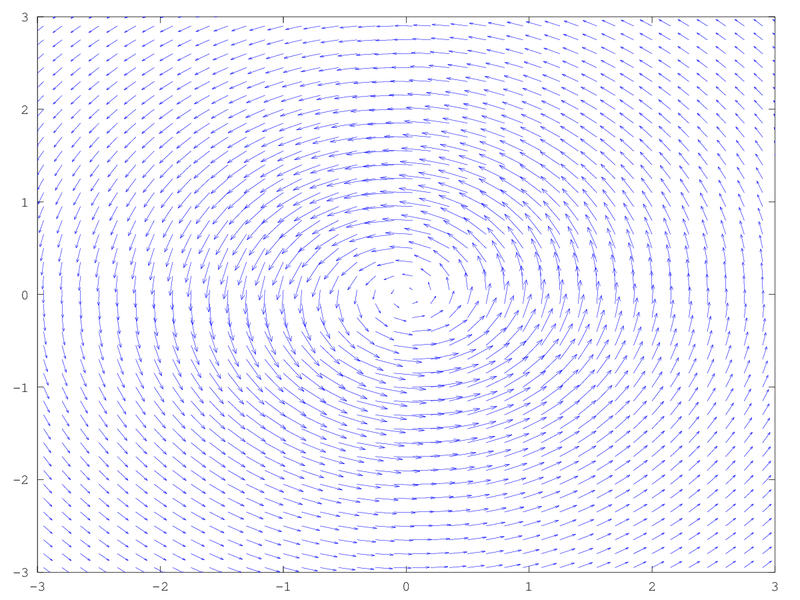
\includegraphics[scale=1]{img/vortex.png}
\caption{Plot of Lamb-Oseen's field.}
\end{figure}

Burgers later a 3D solution:

\begin{equation}
\bm{v} = -\frac{\alpha}{2r}\bm{\hat{r}} + \frac{\Gamma}{2\pi r}\pc{1-\exp\p{-\frac{r^2}{4\nu t}}}\bm{\hat{\theta}} + \alpha\bm{\hat{z}}. 
\end{equation}
It is said \cite{analyticalVSolutions}.

\section{Otros}
\begin{enumerate}
\item La función $\tanh(x/\sqrt{2})$ es solución a la ecuación diferencial:
\begin{equation}
-\lspl{f}{x}(x) + f^3(x) - f(x) = 0,
\end{equation}
pues
\begin{equation*}
-\lspl{}{x}\tanh(x/\sqrt{2}) = \tanh(x/\sqrt{2})\sech^2(x/\sqrt{2}) = \tanh(x/\sqrt{2}) - \tanh^3(x/\sqrt{2}).
\end{equation*}
\end{enumerate}

\section{Personal}
\subsection{Ideas}
\begin{enumerate}
\item Idea para calcular el periodo del vórtice: tomar el máximo de densidad en la red. Leer un semi-plano $\theta = cte$ y ver si en él está un punto con un cierto error.
\item Graficar el promedio de la densidad en el semi-plano anterior con el tiempo. Usar el cambio en la derivada para determinar los máximos.
\end{enumerate}
\subsection{Calendario}
\begin{itemize}
\item Jueves Vórtices clásicos
\item Viernes Electro, Vórtices clásicos
\item Sábado Libre ¿Bogoliubov?
\item Domingo Electro, (Campo de una esfera, etc…), Solución de Gross-Pitaevsky
\end{itemize}

\bibliography{/Users/ole/Documents/bibliografia/bibliography}
\bibliographystyle{plain}

\end{document}